%!TEX program = xelatex

\documentclass[a4paper,12pt]{article}

\usepackage[top=30mm,bottom=25mm,left=25mm,right=25mm]{geometry}
\usepackage{graphicx}
\usepackage{float}
\usepackage{xcolor}
\definecolor{sbublue}{RGB}{31,78,121}
\definecolor{sbublue2}{RGB}{46,116,181}
\usepackage{enumitem}
\usepackage[font=small,labelfont=bf,skip=5pt]{caption}
\usepackage{titlesec}
\usepackage[hidelinks]{hyperref}

\usepackage{xepersian}
\settextfont[BoldFont={IRLotusICEE_Bold.ttf},
             ItalicFont={IRLotusICEE_Iranic.ttf},
             BoldItalicFont={IRLotusICEE_BoldIranic.ttf},
             Scale=1.15]{IRLotusICEE.ttf}
\setlatintextfont[Scale=1.0]{Times New Roman}

\setfootnoteLR

\renewcommand{\figurename}{تصویر}
\renewcommand{\contentsname}{فهرست مطالب}

\titleformat{\section}
  {\normalfont\Large\bfseries\color{sbublue}}{\thesection}{0.6em}{}
\titlespacing{\section}{0pt}{16pt plus 3pt minus 2pt}{6pt}

\linespread{1.45}
\setlength{\parindent}{1em}
\setlength{\parskip}{2pt}

\newlist{terms}{itemize}{1}
\setlist[terms]{label=$\bullet$, leftmargin=1.6em, itemsep=3pt, topsep=3pt, parsep=0pt}
\newcommand{\term}[1]{\textbf{\textcolor{sbublue2}{#1:}}}

\begin{document}
\renewcommand{\figurename}{تصویر}

\begin{titlepage}
\centering
\vspace*{2mm}

\includegraphics[width=3.4cm]{sbu_logo.png}\\[3mm]
{\large\bfseries دانشگاه شهید بهشتی}\\[1.5mm]
{\normalsize دانشکده مهندسی و علوم کامپیوتر}\\[16mm]

{\normalsize\bfseries گزارش فاز اول پروژه‌ی درس سیستم‌های نرم‌افزاری مقیاس‌وسیع \lr{(ULS)}}\\[12mm]

{\LARGE\bfseries\color{sbublue} طراحی و مدل‌سازی فرآیند\\[2mm]
یکپارچه‌سازی سفارش‌های فروشگاه اینترنتی}\\[6mm]

{\normalsize گرایش نرم‌افزار}\\[18mm]

{\large دانشجویان:}\\[1.5mm]
{\large\bfseries شبنم جلیل‌پور}\\[1.5mm]
{\large\bfseries محمدسعید زارع مهرجردی}\\[12mm]

{\large استاد راهنما:}\\[1.5mm]
{\large\bfseries دکتر فریدون شمس}\\[10mm]

\vfill
{\large تیر ۱۴۰۵}
\end{titlepage}

\thispagestyle{empty}
\tableofcontents
\newpage

\setcounter{page}{1}

\section{مقدمه و تبیین مسئله}
در سازمان‌های امروزی، سیستم‌های اطلاعاتی و برنامه‌های کاربردی به دلایل مختلف به‌صورت جزیره‌ای و ناهمگون توسعه یافته‌اند. یکپارچه‌سازی نرم‌افزارهای سازمان\footnote{\lr{Enterprise Application Integration (EAI)}} ابزار و رویکردی است که به این برنامه‌ها اجازه می‌دهد تا فرآیندها و داده‌های خود را با یکدیگر به اشتراک بگذارند.

در این پروژه، سناریوی یک فروشگاه اینترنتی مطرح است که سفارش‌های مشتریان را در قالب فایل‌های متنی (شامل نام مشتری، محصول، تعداد و قیمت) در یک پوشه‌ی ورودی دریافت می‌کند. هدف فاز اول، طراحی و مدل‌سازی معماری این سیستم است، طوری که عملیات خواندن، غنی‌سازی داده (افزودن زمان دریافت\footnote{\lr{Timestamp}})، اعتبارسنجی، مدیریت خطاهای احتمالی و گزارش‌دهی دوره‌ای وضعیت سیستم را به‌صورت کاملا خودکار، بدون توقف و مبتنی بر الگوهای استاندارد یکپارچه‌سازی سازمانی\footnote{\lr{Enterprise Integration Patterns (EIP)}} انجام دهد.

\section{تعیین سبک و سطح یکپارچه‌سازی}
بر اساس مفاهیم پایه‌ی درس، چهار سبک اصلی برای یکپارچه‌سازی وجود دارد:
\begin{terms}
  \item انتقال فایل\footnote{\lr{File Transfer}}
  \item پایگاه‌داده‌ی مشترک\footnote{\lr{Shared Database}}
  \item فراخوانی رویه از راه دور\footnote{\lr{Remote Procedure Call (RPC)}}
  \item پیام‌رسانی\footnote{\lr{Messaging}}
\end{terms}
این پروژه در سطح داده و بر پایه‌ی ترکیبی از دو سبک معماری طراحی شده است:
\begin{terms}
  \item \term{سبک انتقال فایل} بستر فیزیکی تبادل داده‌ها بر اساس فایل است. سیستم‌های بیرونی سفارش‌ها را در پوشه‌ی ورودی می‌نویسند و خروجی نیز در قالب فایل ذخیره می‌شود. این سبک، عدم وابستگی زمانی و مکانی مناسبی ایجاد می‌کند.
  \item \term{سبک پیام‌رسانی} برای پیاده‌سازی داخلی لایه‌ی میانی، از دیدگاه پیام‌رسانی استفاده شده است. چارچوب \lr{Apache Camel} هر فایل ورودی را یک پیام و مسیرهای پردازش را کانال پیام در نظر می‌گیرد. با این ترکیب می‌توانیم از مزایای اتصال سست\footnote{\lr{Loose Coupling}} در این بستر استفاده کنیم.
\end{terms}

\section{معماری سیستم و الگوهای مسیریابی}
ساختار اصلی پردازش سفارش‌ها در این سیستم بر اساس الگوی لوله‌ها و فیلترها\footnote{\lr{Pipes and Filters}} مدل‌سازی شده است. در این الگو، هر گام پردازشی یک فیلتر مستقل است و پیام‌ها از طریق کانال‌ها بین این فیلترها جریان دارند. نمای کلی این معماری در تصویر~\ref{fig:dfd} نشان داده شده است.

\begin{figure}[H]
  \centering
  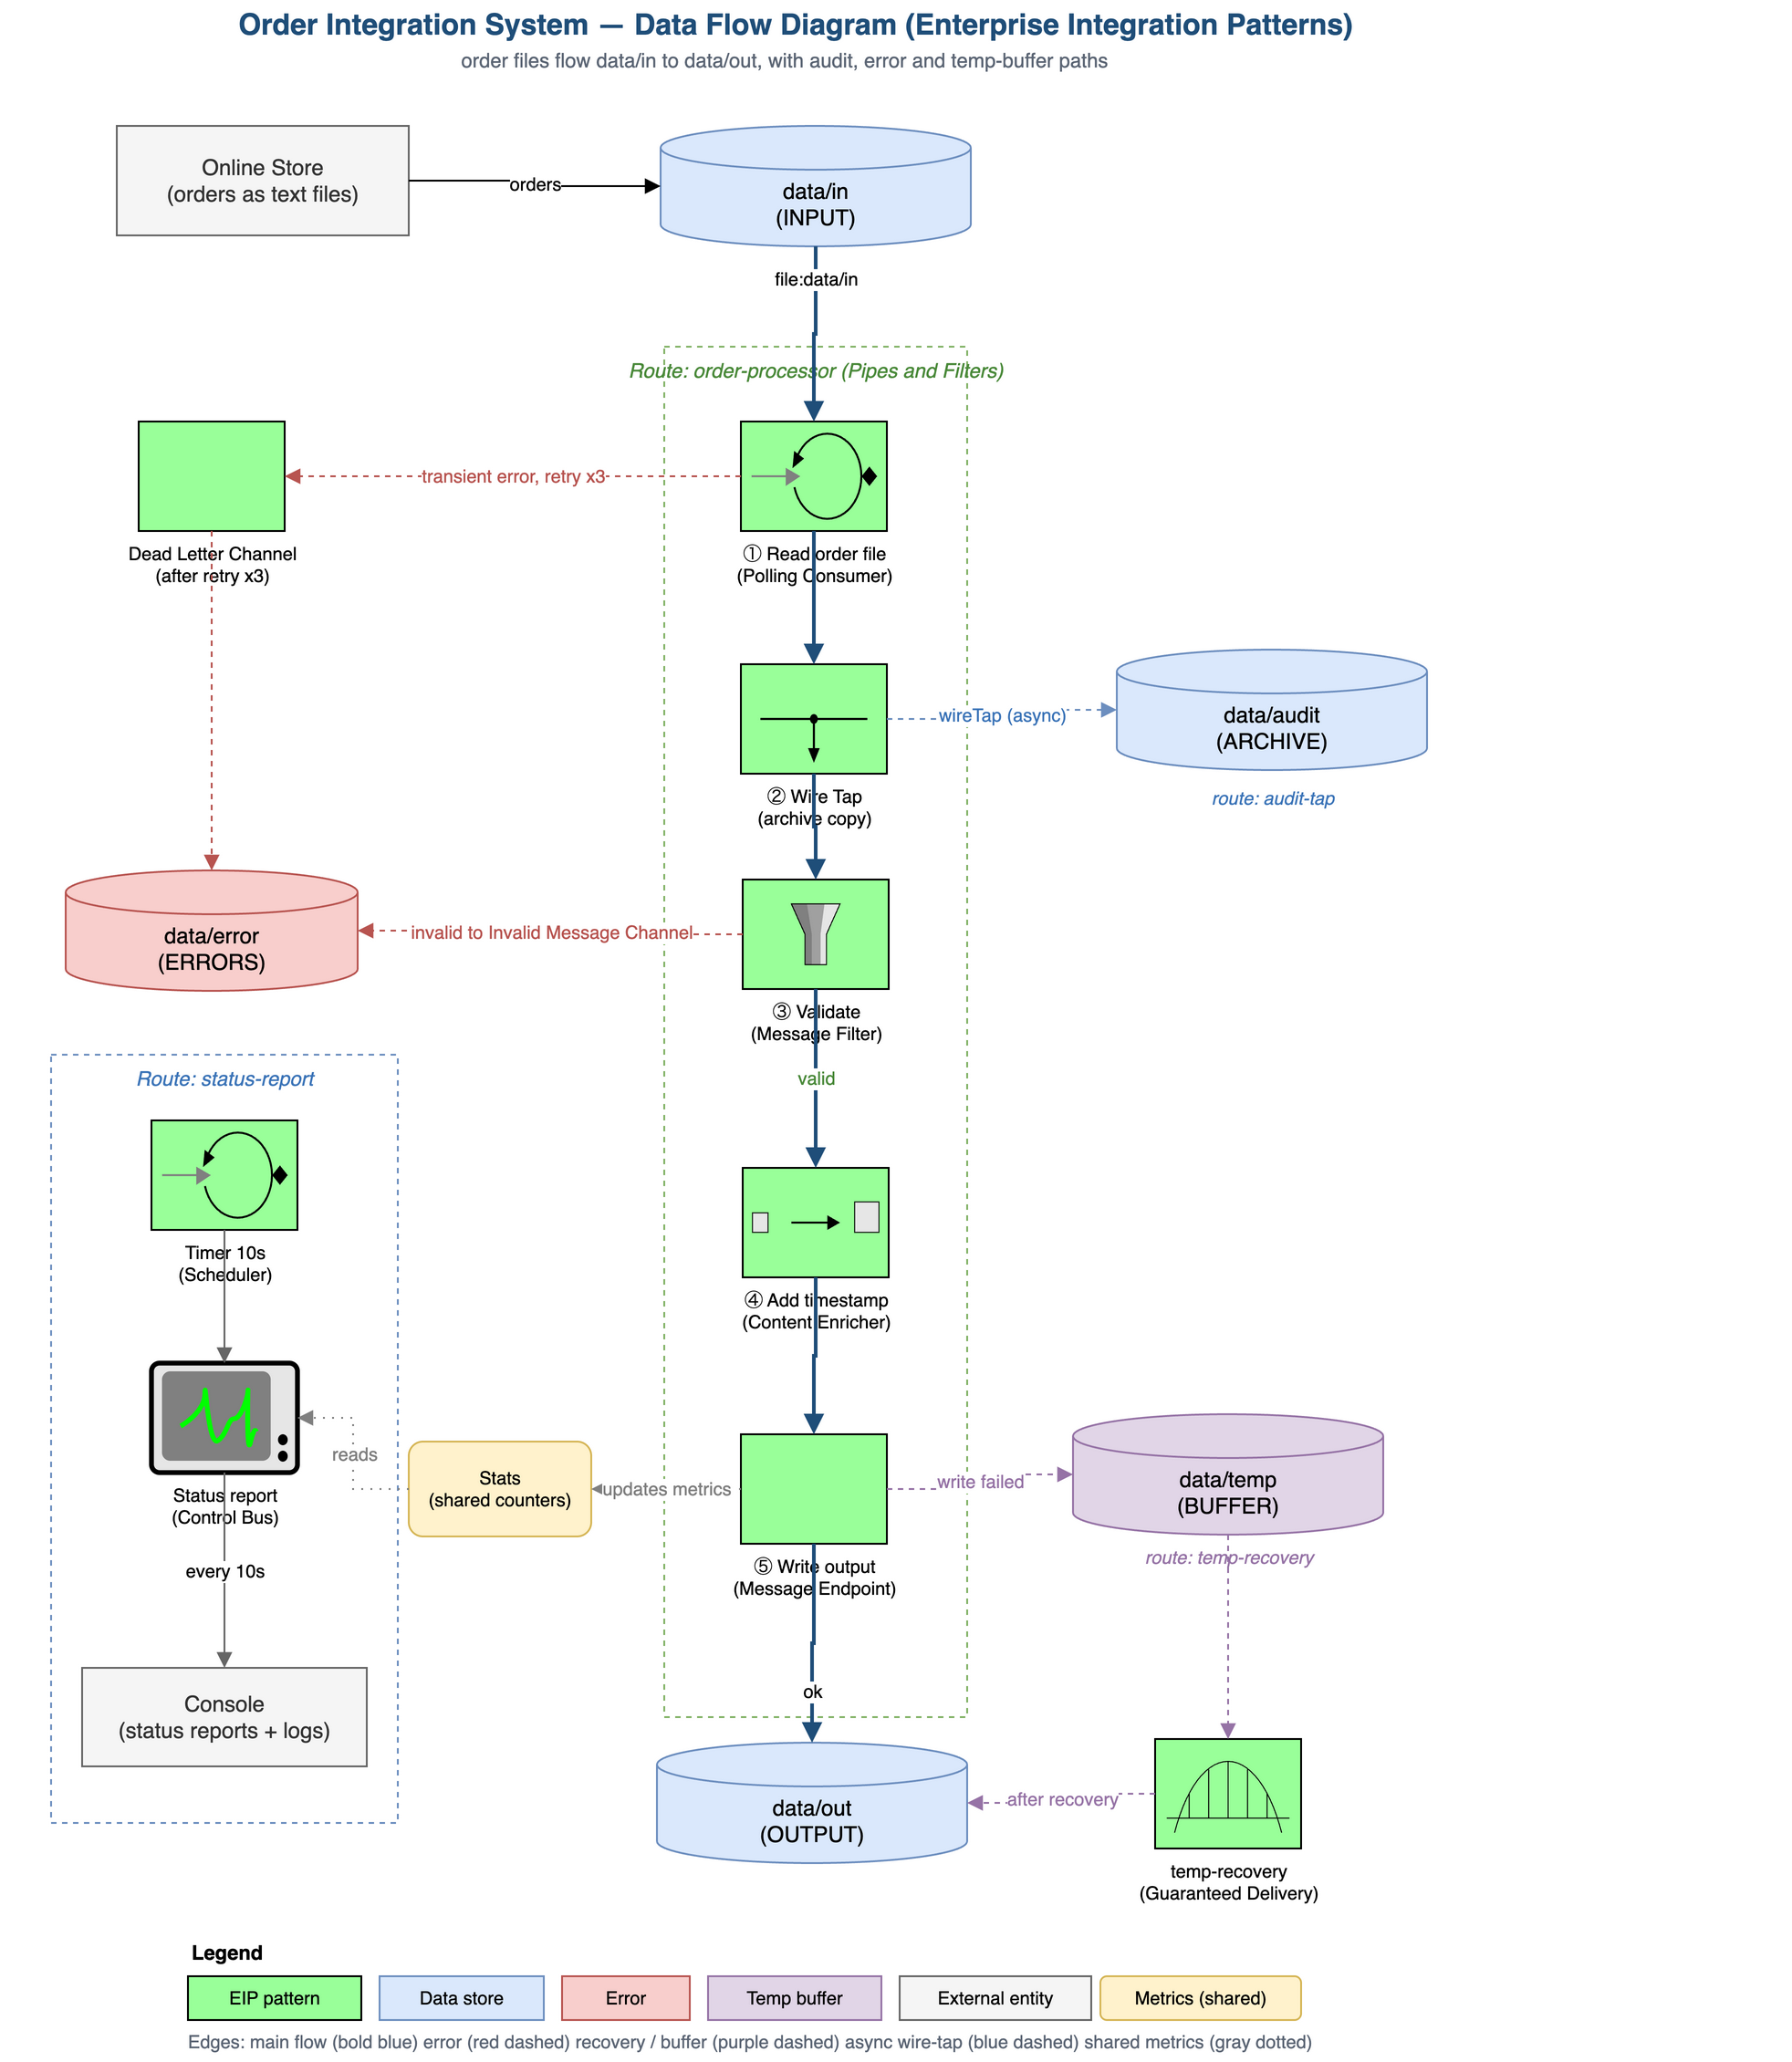
\includegraphics[width=0.84\textwidth]{dfd.png}
  \caption{نمودار جریان داده‌ی فرآیند یکپارچه‌سازی سفارش‌های فروشگاه اینترنتی (حاشیه‌نویسی‌شده با الگوهای \lr{EIP})}
  \label{fig:dfd}
\end{figure}

همان‌طور که در نمودار بالا مشاهده می‌شود، مؤلفه‌ها و فیلترهای اصلی این سیستم عبارت‌اند از:
\begin{terms}
  \item \term{مصرف‌کننده‌ی دوره‌ای}\footnote{\lr{Polling Consumer}} سیستم به‌صورت دوره‌ای پوشه‌ی ورودی (\lr{data/in}) را سرکشی کرده و به‌محض یافتن فایل جدید، آن را به‌عنوان یک پیام وارد سیستم می‌کند.
  \item \term{شنود پیام}\footnote{\lr{Wire Tap}} برای نگه‌داشتن سابقه، درست پس از خواندن فایل و پیش از اعتبارسنجی و غنی‌سازی، یک کپی از پیام به‌صورت ناهمگام به پوشه‌ی بایگانی (\lr{data/audit}) فرستاده می‌شود تا از همه‌ی پیام‌های دریافتی یک لاگ داشته باشیم. این پوشه یک انتخاب طراحی اختیاری است و چون کپی ناهمگام انجام می‌شود، مسیر اصلی را کند نمی‌کند.
  \item \term{اعتبارسنجی و فیلتر پیام}\footnote{\lr{Message Filter}} این مؤلفه کار اعتبارسنجی را انجام می‌دهد. در صورتی که فایل ورودی خالی یا ناقص باشد، پیام نامعتبر شناخته شده و از طریق الگوی کانال پیام‌های نامعتبر\footnote{\lr{Invalid Message Channel}} به پوشه‌ی \lr{data/error} هدایت می‌شود؛ در غیر این صورت به گام بعد می‌رود.
  \item \term{غنی‌ساز پیام}\footnote{\lr{Content Enricher}} سفارش‌های معتبر وارد این گام می‌شوند. سیستم زمان دریافت را از ساعت داخلی سرور (به‌عنوان منبع غنی‌سازی از محیط) می‌گیرد و به محتوای پیام اضافه می‌کند.
  \item \term{نقطه‌ی پایانی پیام}\footnote{\lr{Message Endpoint}} در نهایت، پیام غنی‌شده به پوشه‌ی خروجی (\lr{data/out}) که نقطه‌ی پایانی سیستم است منتقل و ذخیره می‌شود.
  \item \term{تحویل تضمین‌شده}\footnote{\lr{Guaranteed Delivery}} در صورت خطای خروجی، داده‌ها در پوشه‌ی موقت (\lr{data/temp}) ذخیره می‌شوند و مسیر \lr{temp-recovery} پس از رفع مشکل آن‌ها را به پوشه‌ی خروجی برمی‌گرداند.
  \item \term{پایش و گزارش‌گیری}\footnote{\lr{Control Bus}} سرویسی موازی با فرآیند اصلی که برای نظارت، هر ۱۰ ثانیه گزارش وضعیت سامانه را در کنسول چاپ می‌کند.
\end{terms}

دو مسیر خطای این سیستم — کانال پیام‌های نامعتبر (برای فایل‌های خالی یا ناقص) و کانال پیام‌های مرده (برای خطاهای موقت پس از سه تلاش) — دو الگوی جدا هستند که در عمل در یک پوشه‌ی واحد (\lr{data/error}) کنار هم قرار می‌گیرند. جزئیات این دو، همراه با جعبه‌های \lr{Dead Letter Channel} و \lr{temp-recovery} در نمودار، در بخش تحلیل سناریوهای خطا توضیح داده شده است.

\section{سرویس‌ها و نقاط اتصال میان آن‌ها}
سیستم از سه سرویس تشکیل شده که چارچوب \lr{Apache Camel} آن‌ها را به هم وصل و با هم هماهنگ می‌کند:
\begin{terms}
  \item \term{سرویس فایل} مسئول خواندن سفارش‌ها از پوشه‌ی ورودی (\lr{data/in}) و نوشتن خروجی در پوشه‌های \lr{data/out}، \lr{data/audit}، \lr{data/error} و \lr{data/temp} است. نقاط اتصال این سرویس، نقاط پایانی فایل\footnote{\lr{File Endpoints}} در ابتدا و انتهای مسیرها هستند.
  \item \term{سرویس پردازشگر} منطق اعتبارسنجی و غنی‌سازی (افزودن زمان دریافت) را اجرا می‌کند و در میانه‌ی مسیر \lr{order-processor} از طریق کانال‌های داخلی به سرویس فایل متصل می‌شود.
  \item \term{سرویس زمان‌بندی} مسیر مستقل \lr{status-report} را اجرا می‌کند و از طریق گذرگاه کنترل، خروجی‌اش را در کنسول نمایش می‌دهد.
\end{terms}
دو وابستگی اصلی هم وجود دارد: مسیر \lr{audit-tap} که از طریق کانال مستقیم\footnote{\lr{direct:audit}} به سرویس فایل وصل است، و مسیر \lr{temp-recovery} که میان پوشه‌ی موقت و پوشه‌ی خروجی رابط است. سرویس زمان‌بندی از دو سرویس دیگر مستقل است و فقط شمارنده‌های مشترک را می‌خواند؛ همین اتصال سست باعث می‌شود پردازش در برابر خطاها بدون توقف ادامه پیدا کند.

\section{تحلیل سناریوهای خطا و افزایش تاب‌آوری}
برای پایدارماندن در مقیاس وسیع، سیستم سه سناریوی خطا را با کمک الگوهای \lr{EIP} مدیریت می‌کند:
\begin{terms}
  \item \term{تأخیر یا خطای موقت در خواندن} در صورت بروز تأخیر یا خطای موقت هنگام خواندن فایل، سازوکار تحویل مجدد\footnote{\lr{Retry / Redelivery}} تا ۳ بار تلاش می‌کند؛ در صورت تداوم خطا، پیام بدون متوقف‌کردن سیستم به کانال پیام‌های مرده در \lr{data/error} منتقل می‌شود.
  \item \term{عدم دسترسی به پوشه‌ی خروجی} در صورت شکست در نوشتن روی پوشه‌ی خروجی، داده‌ها در پوشه‌ی موقت (\lr{data/temp}) ذخیره می‌شوند. فایل تا زمانی که پوشه‌ی خروجی در دسترس نباشد در \lr{data/temp} باقی می‌ماند و در هر چرخه‌ی بازیابی مجددا تلاش می‌شود؛ پس از رفع مشکل، به مسیر اصلی بازمی‌گردد.
  \item \term{فایل خالی یا ناقص} توسط الگوی کانال پیام‌های نامعتبر\footnote{\lr{Invalid Message Channel}}، این فایل‌ها جداسازی شده و مستقیما به پوشه‌ی خطا فرستاده می‌شوند تا پردازش سایر فایل‌ها بدون وقفه ادامه یابد.
\end{terms}

\section{پایش سیستم و گذرگاه کنترل}
برای نظارت بر سلامت و کارایی سیستم، یک فرآیند موازی و مستقل بر پایه‌ی الگوی گذرگاه کنترل طراحی شده است. این سرویس به کمک یک کامپوننت تایمر، هر ۱۰ ثانیه یک‌بار فعال شده و معیارهای حیاتی سیستم (تعداد فایل‌های موفق، ناموفق و موقت) را که در شمارنده‌های ایمن از نظر هم‌روندی ذخیره شده‌اند، در کنسول نمایش می‌دهد تا مدیران سیستم از زنده‌بودن فرآیند مطمئن شوند.

نکته این است که مسیر پایش و مسیر پردازش هیچ کانال پیامی با هم ندارند و کاملا مستقل‌اند؛ تنها راه ارتباطشان همین شمارنده‌های مشترک است که در نمودار با عنصر \lr{Stats} نشان داده شده: مسیر پردازش این شمارنده‌ها را به‌روزرسانی می‌کند و مسیر پایش آن‌ها را می‌خواند. چون این ارتباط از جنس حالت مشترک است و نه پیام، در نمودار به‌جای کانال پیام با یال‌های نقطه‌چین خاکستری رسم شده است. همین جدایی باعث می‌شود پایش حتی وقتی مسیر اصلی متوقف یا کند شود باز هم کار کند و زنده‌بودن سامانه را گزارش دهد — که دقیقا هدف الگوی گذرگاه کنترل است.

\section{جمع‌بندی}
در این فاز از پروژه، سناریوی فروشگاه اینترنتی به‌عنوان یک یکپارچه‌سازی درون‌سازمانی\footnote{\lr{Application-to-Application (A2A)}} در سطح داده و بر پایه‌ی رویکرد استخراج، تبدیل و بارگذاری\footnote{\lr{Extract, Transform, Load (ETL)}} مدل‌سازی شد. این معماری، ترکیبی از بستر فیزیکی انتقال فایل و منطق پیام‌رسانی است که با چارچوب \lr{Apache Camel} مدیریت می‌شود. خروجی‌های این فاز — نمودار جریان داده، شناسایی مؤلفه‌ها و کانال‌های ارتباطی، و همین گزارش توصیفی — پایه‌ی مستقیم پیاده‌سازی فاز دوم را فراهم می‌کنند.

\end{document}
